\newpage
\section{Diagramas de secuencia}
A continuación se describe la interacción de nuestras entidades de negocio y el ciclo de vida que tendrán en la aplicación. También se detalla la interacción, mensajes y la lógica implementada en cada uno de los diferentes escenarios.\par

\subsection{DS1. Inicio de sesión}
El inicio de sesión consiste en la captura de usuario y contraseña de una cuenta para tener acceso a sus datos. Estos dos datos se envían en formato JSON a AWS API Gateway que sirve de puerta de enlace para poder establecer una comunicación con la AWS Lambda \textit{ARFLogin} la cual se encarga de realizar una consulta en una base de datos en MySQL montada sobre una instancia de AWS RDS para verificar que los datos correspondan a una cuenta registrada. El resultado de esta consulta, ya sea exitosa o fallida, se devuelve a ARF en formato JSON a través de AWS API Gateway. Esta respuesta tiene dos parámetros que indican el estatus de la operación: \textbf{code} y \textbf{message}

\begin{figure}[h!]
	\centering
	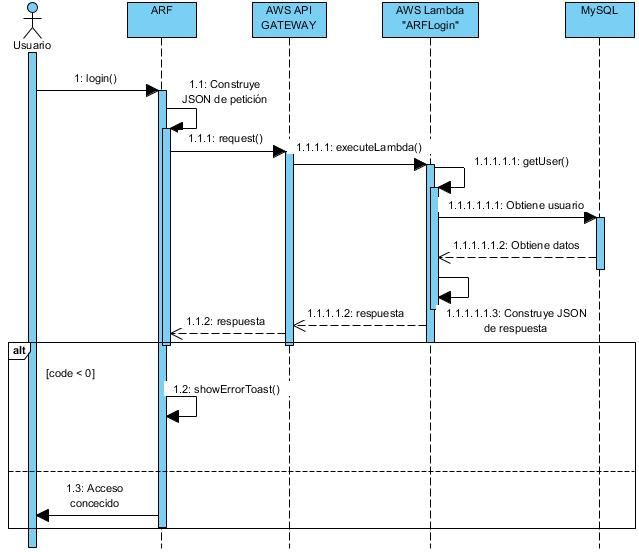
\includegraphics[width=14cm,height=14cm]{imagenes/analisis/ds/dsinicio_sesion.jpg}
	\caption{DS1. Inicio de sesión.}
	\label{fig:dsiniciosesion}
\end{figure}

\clearpage

\subsection{DS2. Registro de cuenta}
El registro de cuenta consiste en la captura de nombre, email y contraseña. La contraseña se deberá repetir. Esos datos se envían en formato JSON a AWS API Gateway la cual se encarga de ejecutar la AWS Lambda \textit{ARFRegisterAccount}. Esta función se encarga primero de consultar el correo para verificar que se cumpla la regla de negocio \textbf{BR1}. Si la regla se cumple, entonces el usuario es registrado por esta función. Ya sea que la inserción sea realizado con éxito o no, la función construye nu JSON de respuesta que contiene el status de la operación, y esta respuesta es manipulada por la aplicación para mostrar en pantalla un error, o redirigir el usuario a la pantalla de Inicio de sesión.

\begin{figure}[h!]
	\centering
	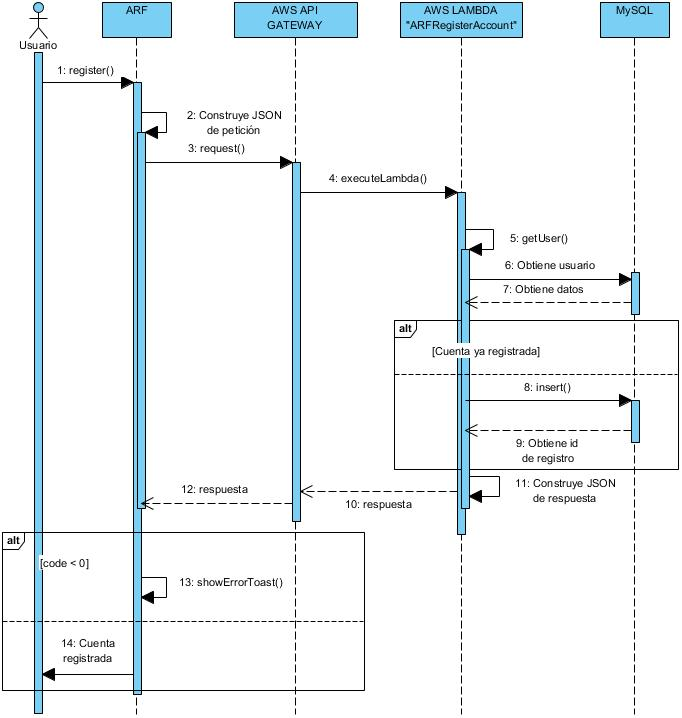
\includegraphics[width=14cm,height=16cm]{imagenes/analisis/ds/RegCuenta.jpg}
	\caption{DS2. Registro de cuenta.}
	\label{fig:dsregcuenta}
\end{figure}
\clearpage

\subsection{DS3. Recuperación de cuenta}
El proceso de recuperación se divide en tres pasos:
\begin{itemize}
	\item \textbf{Envío de código:} El usuario introduce el email de su cuenta, la aplicación se comunica con la AWS Lambda \textit{ARFRecoverAccount} a través de la AWS API Gateway con mensajes en formato JSON. La Lambda se encarga de verificar que el email pertenezca a una cuenta registrada. De ser así, se envía un email a tal cuenta con un código de verificación generado para esa cuenta, en otro caso se muestra un mensaje del error. La función responde en JSON indicando el estatus de esta operación. De ser exitosa, la pantalla de \textit{Verificación de código}.
	\item \textbf{Verificación de código:} El usuario ingresa el código que fue enviado a su correo. De nuevo se realiza la comunicación a la AWS Lambda \textit{ARFRecoverAccount} via AWS API Gateway. La función se encarga de validar que el código ingresado por el usuario corresponda al que se generó y envió previamente. La Lambda responde con el status de esta validación. Si la validación es correcta, la aplicación muestra la pantalla de \textit{Reestablecimiento de contraseña}, en caso contrario muestra un mensaje describiendo el error.
	\item \textbf{Reestablecimiento de contraseña:} El usuario captura la nueva contraseña que desea que tenga su cuenta. De nuevo se realiza la comunicación a la AWS Lambda \textit{ARFRecoverAccount} via AWS API Gateway. La función se encarga de actualizar en la base de datos la contraseña del usuario, y responde con el status de esta operación. Finalmente el usuario es redireccionado al Inicio de sesión para poder acceder a su cuenta con la nueva contraseña.
\end{itemize}

\begin{figure}[h!]
	\centering
	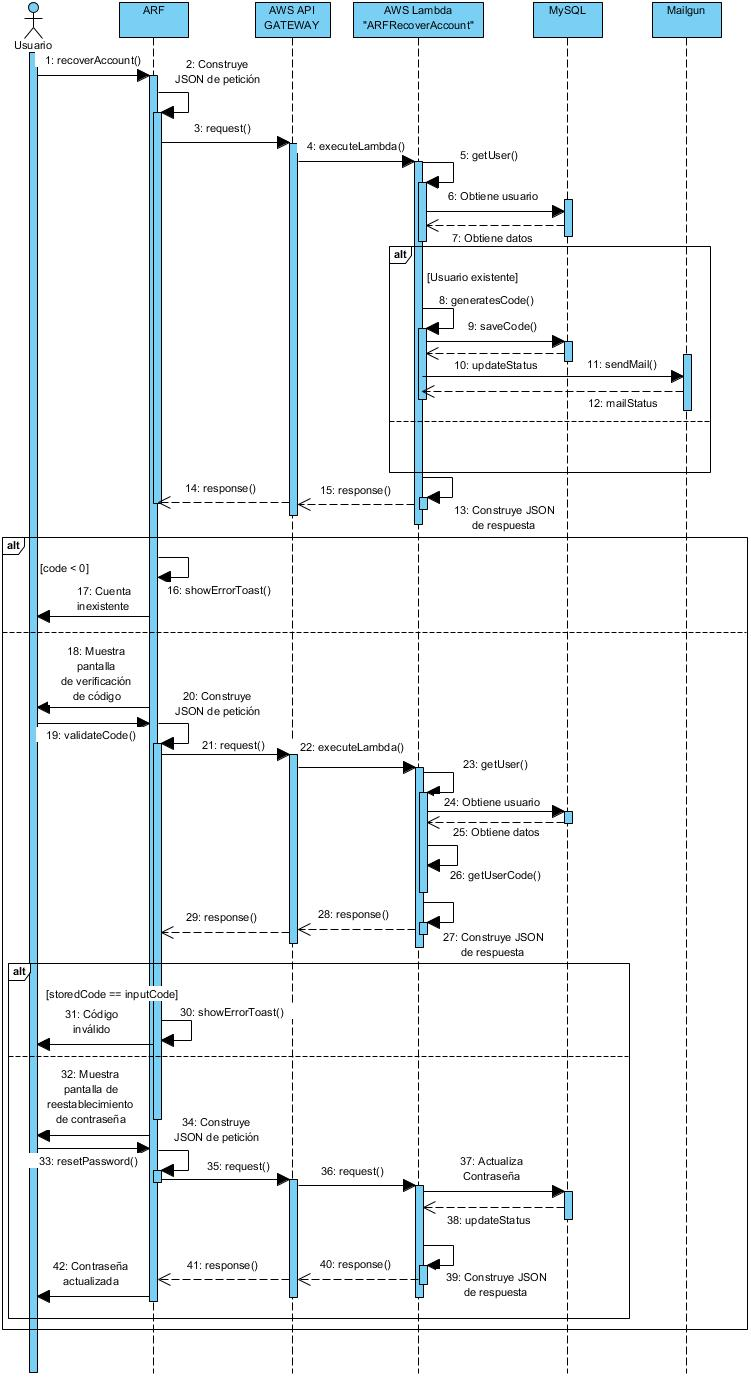
\includegraphics[width=13cm,height=22cm]{imagenes/analisis/ds/RecCuenta.jpg}
	\caption{DS3. Recuperación de cuenta.}
	\label{fig:dsreccuenta}
\end{figure}
\clearpage

\subsection{DS4. Gestión de proyectos}
Aquí se presentan cinco escenarios: creación de proyecto, actualización de proyecto, eliminación de proyecto, obtención de proyecto, y obtención de proyectos de usuario.
\begin{itemize}
	\item \textbf{Creación de proyecto:} El usuario llena un formulario donde le pide datos del cliente del proyecto (nombre, apellido y  teléfono). Tras llenarlos y seleccionar \textit{Crear proyecto}, la aplicación envía estos datos a la AWS Lambda \textit{ARFProject} en formato JSON a través de la AWS API Gateway, la cual se encarga de hacer la inserción del proyecto en la base da datos con base en los datos recibidos y responde con el status de tal operación. La aplicación recibe esta respuesta y muestra un mensaje con error en caso de haberlo o redirige al usuario a la pantalla de \textit{Visualización de escenarios} donde ya se muestra el proyecto que acaba de generar.
	\item \textbf{Actualización del proyecto: } Dentro de un proyecto el usuario modifca los campos que desee actualizar y selecciona \textit{Actualizar}. Estos datos se envían en formato JSON a la AWS Lambda \textit{ARFProject} via AWS API Gateway, la cual se encarga de actualizar en la base de datos el proyecto correspondiente de acuerdo a la información recibida y responde con el status de tal operación. La aplicación recibe esta respuesta y muestra un mensaje con error en caso de haberlo o redirige al usuario a la pantalla de \textit{Visualización de proyectos}.
	\item \textbf{Eliminación de proyecto:} El usuario selecciona el icono de eliminación de alguno de los proyectos listados. La aplicación se comunica a la AWS Lambda \textit{ARFProject} via AWS API Gateway, la cual se encarga de hacer la eliminación del proyecto solicitado en la base de datos y responde con el status de tal operación. La aplicación recibe esta respuesta y muestra un mensaje con error en caso de haberlo o redirige al usuario a la pantalla de \textit{Visualización de proyectos}.
	\item \textbf{Obtención de proyecto:} Cuando el usuario selecciona un proyecto para visualizar su información, se hace una petición a la AWS Lambda \textit{ARFProject} para obtener la información completa del proyecto en cuestión desde la base de datos y la Lambda responde con el proyecto solicitado. Finalmente la aplicación muestra los datos recibidos a través de un formulario que permitirá actualizar el proyecto.
	\item \textbf{Obtención de proyectos de usuario:} Cuando un usuario entra a la pantalla de \textit{Visualización de proyectos} se hace una petición a la AWS Lambda \textit{ARFProject} via AWS API Gateway, la función se encarga de obtener de la base de datos todos los proyectos que pertenezcan al usuario que realiza la solicitud y responde con esta información. Finalmente la aplicación recibe esta respuesta y despliega un listado de los proyectos obtenidos.
\end{itemize}

\begin{figure}[h!]
	\centering
	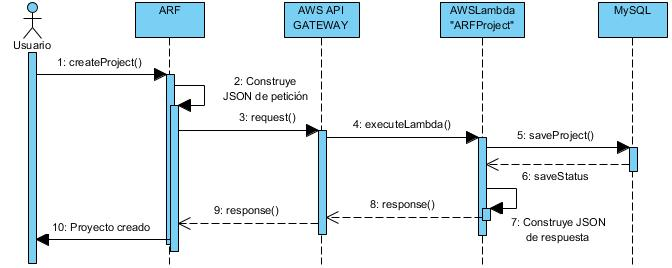
\includegraphics[width=14cm,height=8cm]{imagenes/analisis/ds/CreateProject.jpg}
	\caption{DS4. Gestión de proyectos.}
	\label{fig:dsreccuenta}
\end{figure}
\clearpage


\subsection{DS5. Gestión de escenarios}
Aquí se presentan cinco escenarios: creación de escenario, actualización de escenario, eliminación de escenario, obtención de escenario, y obtención de escenarios de proyecto.
\begin{itemize}
	\item \textbf{Creación de escenario:} Tras finalizar la creación del entorno de realidad aumentada y haber tomado las fotografías deseadas, el usuario confirma la creación de un proyecto, entonces la aplicación se comunica con la AWS Lambda \textit{ARFScenario} via AWS API Gateway, a la cual le envía la información general del escenario y las fotografías y videos realizados. Esta función se encarga de almacenar en AWS S3 los archivos recibidos y generar un registro de escenario en la base de datos que también asocie estos recursos almacenados a través de su URL pública de descarga. Tras esto, la función responde con el registro del escenario creado. La aplicación recibe esta respuesta y regresa a la pantalla de \textit{Visualización de escenarios} y muestra un mensaje de error en caso de haberlo.
	\item \textbf{Actualización de escenario: } Dentro de un escenario el usuario modifca los campos que desee actualizar y selecciona \textit{Actualizar}. Estos datos se envían en formato JSON a la AWS Lambda \textit{ARFScenario} via AWS API Gateway, la cual se encarga de actualizar en la base de datos el escenario correspondiente de acuerdo a la información recibida y responde con el status de tal operación. La aplicación recibe esta respuesta y muestra un mensaje con error en caso de haberlo o redirige al usuario a la pantalla de \textit{Visualización de escenarios}.
	\item \textbf{Eliminación de escenario:} El usuario selecciona el icono de eliminación de alguno de los escenario listados. La aplicación se comunica a la AWS Lambda \textit{ARFScenario} via AWS API Gateway, la cual se encarga de hacer la eliminación del escenario solicitado en la base de datos y responde con el status de tal operación. La aplicación recibe esta respuesta y muestra un mensaje con error en caso de haberlo o redirige al usuario a la pantalla de \textit{Visualización de escenarios}.
	\item \textbf{Obtención de escenario:} Cuando el usuario selecciona un escenario para visualizar su información, se hace una petición a la AWS Lambda \textit{ARFScenario} para obtener la información completa del escenario en cuestión desde la base de datos y la Lambda responde con el escenario solicitado. Finalmente la aplicación muestra los datos recibidos a través de un formulario que permitirá actualizar el escenario.
	\item \textbf{Obtención de escenarios de usuario:} Cuando un usuario entra a la pantalla de \textit{Visualización de escenarios} se hace una petición a la AWS Lambda \textit{ARFScenario} via AWS API Gateway, la función se encarga de obtener de la base de datos todos los escenarios que pertenezcan al usuario que realiza la solicitud y responde con esta información. Finalmente la aplicación recibe esta respuesta y despliega un listado de los escenarios obtenidos.
\end{itemize}

\begin{figure}[h!]
	\centering
	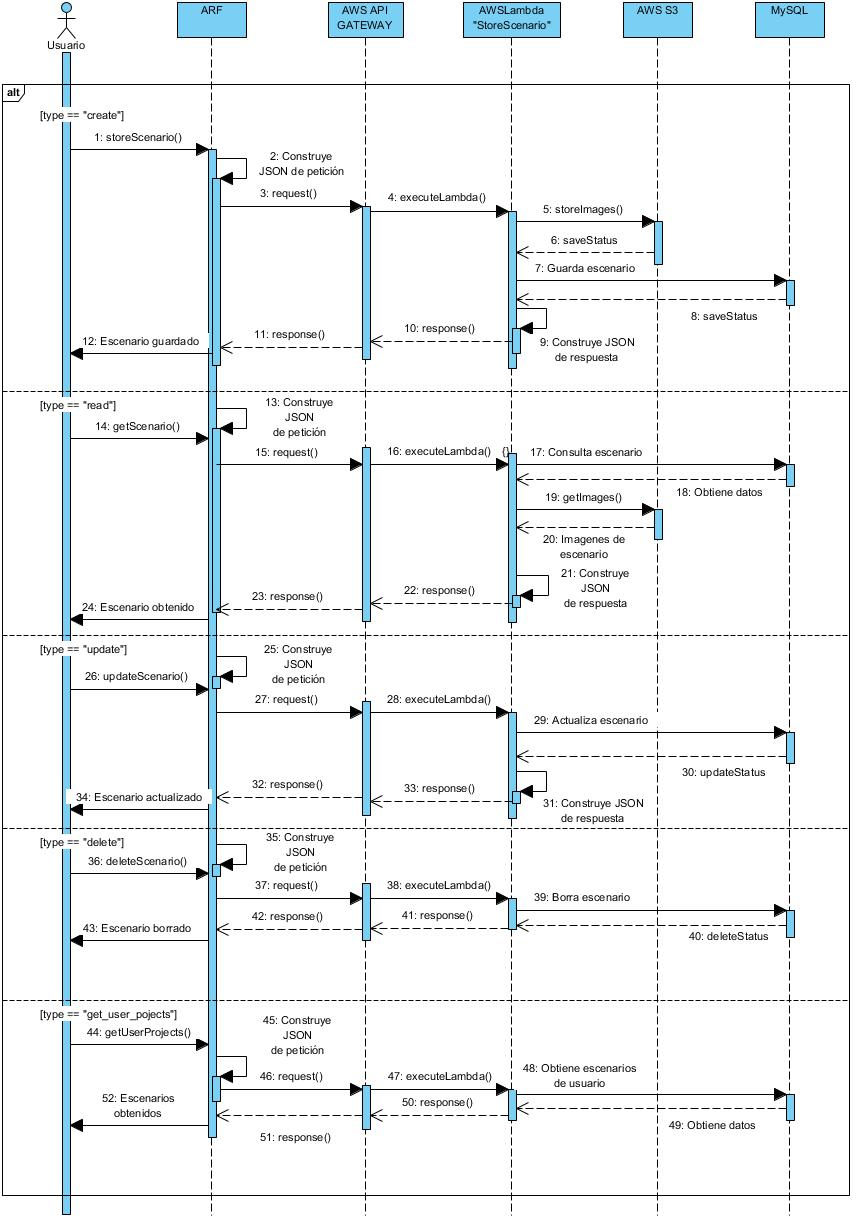
\includegraphics[width=14cm,height=20cm]{imagenes/analisis/ds/CrearEscenario.jpg}
	\caption{DS5. Gestión de escenarios.}
	\label{fig:dsreccuenta}
\end{figure}
\clearpage